\chapter{Particle Identification}\label{chapter:PID}

\section{Introduction}
Following on from the process of clustering hits together into associated groups, and fitting tracks to obtain parameters such as the slope or particle momentum, it is essential to be able to determine the nature of the particle that produced those hits.

For \ac{CCQE} neutrino interactions it is of critical importance to be able to identify the flavour of the lepton that was produced, and to be able to associate a track with the passage of a muon (if the interaction involved a $\nu_\mu$). Muon identification is often performed with the help of small detector units around the sides of the main detector. A muon typically behaves as a minimum ionising particle, and will often travel all the way through a detector and leave through one of the sides. A signal in such a muon detector is a strong indicator that the track leading into it was produced by a muon.

In the case of a \ac{LAr TPC}, the aim is to fully contain muons (at least, if they are produced somewhere near the centre of the detector volume), and identification must be performed using information from the track reconstruction stage. For the simplest category of charged current interactions, the muon should be represented by the longest track visible in the event, and it is on this basis that the primary identification of muon tracks will be carried out.

For other types of interaction, or for electron neutrinos, there is a much greater chance of an electromagnetic or hadronic shower developing in the event. One advantage often claimed of LAr TPCs is the ability to achieve electron--pion separation by looking at the rate of energy loss, $dE/dx$. Attempts at particle identification based on the properties of electromagnetic or hadronic showers are not considered here, but see \citep{Ramachers2012} for details of one such analysis. Since the homogeneous nature of LAr TPCs allows for the coexistence of tracks and showers, a full analysis framework must be able to cope with showers, in addition to tracks. Furthermore, in order to be applicable to $\nu_e$ events, it must be possible to identify electromagnetic showers and obtain calorimetric information from them, in order to be able to estimate the energy of the incoming $\nu_e$. This is an area in which LAr TPCs should excel, but the focus of this thesis is on track reconstruction techniques; an already difficult area for fully automated reconstruction in such a fine-grained environment.

\section{Muon Track Identification}
In order to be able to select muons based on the track length (approximated as the number of hits contained), it is useful to know the distributions of track lengths for various particle types which may be present in the charged current interactions considered. 

% ************ 0.77 GeV CCQE ************
\subsection{$770\MeV$ $\nu_\mu \rightarrow \ccqe$ (CCQE) Interactions}
This study begins by looking at those distributions for the products of charged current interactions of $770\MeV$ $\nu_\mu$ which produced $\ccqe$ or $\ccpi$ final states, making use of the truth information saved by the simulation. Figure \ref{fig:ccqe-track-lengths-770MeV} shows the distribution of lengths (in terms of number of hits) for muon and proton tracks, and figure \ref{fig:ccqe-electron-lengths-770MeV} shows the distribution of lengths for electron tracks, which are plotted on a different graph because the total number of electron tracks is extremely large, though nearly all such tracks have fewer than 50 hits. These correspond to the delta electrons produced along the length of the other tracks. At neutrino energies around $770\MeV$, there is a strong case to be made for treating all tracks longer than $1000$ hits as muons, resulting in a trade-off between selection efficiency for muons and contamination by protons.

\begin{table}
\centering
\begin{tabular}{*{5}{r}}
 & $\mu$ & $p$ & $e^-$ & $\pi^\pm$ \\
\hline
\hline
Included & 960 & 57 & 0 & 0 \\
Excluded & 40 & 1143 & 67228 & 3 \\
\hline
\end{tabular}
\caption[Composition of tracks after $1000$ hit cut on $770\MeV$ CCQE events]{\label{table:cut-results-ccqe-0.77}Composition of tracks after applying a $1000$ hit cut on the truth tracks from simulation of $770\MeV$ $\nu_\mu$ interactions producing $\ccqe$ final states. The cut selects muon tracks with $96.0\pm0.6\%$ efficiency and $94.4\pm0.8\%$ purity.}
\end{table}

Table \ref{table:cut-results-ccqe-0.77} shows the number of tracks included and excluded by a $1000$ hit cut, where the track type is determined from truth information. Since the electron tracks are produced arbitrarily along the muon track, it is impossible to eliminate electron hits from the muon track, even with clustering techniques such as those provided by the cellular automaton (see chapter \ref{chapter:CellularAutomaton}). The purity of any such tracks will therefore be reduced by the presence of hits from these short delta electron tracks, i.e. reconstructed muon tracks will not be $100\%$ pure at the hit level.


\begin{figure}
\centering
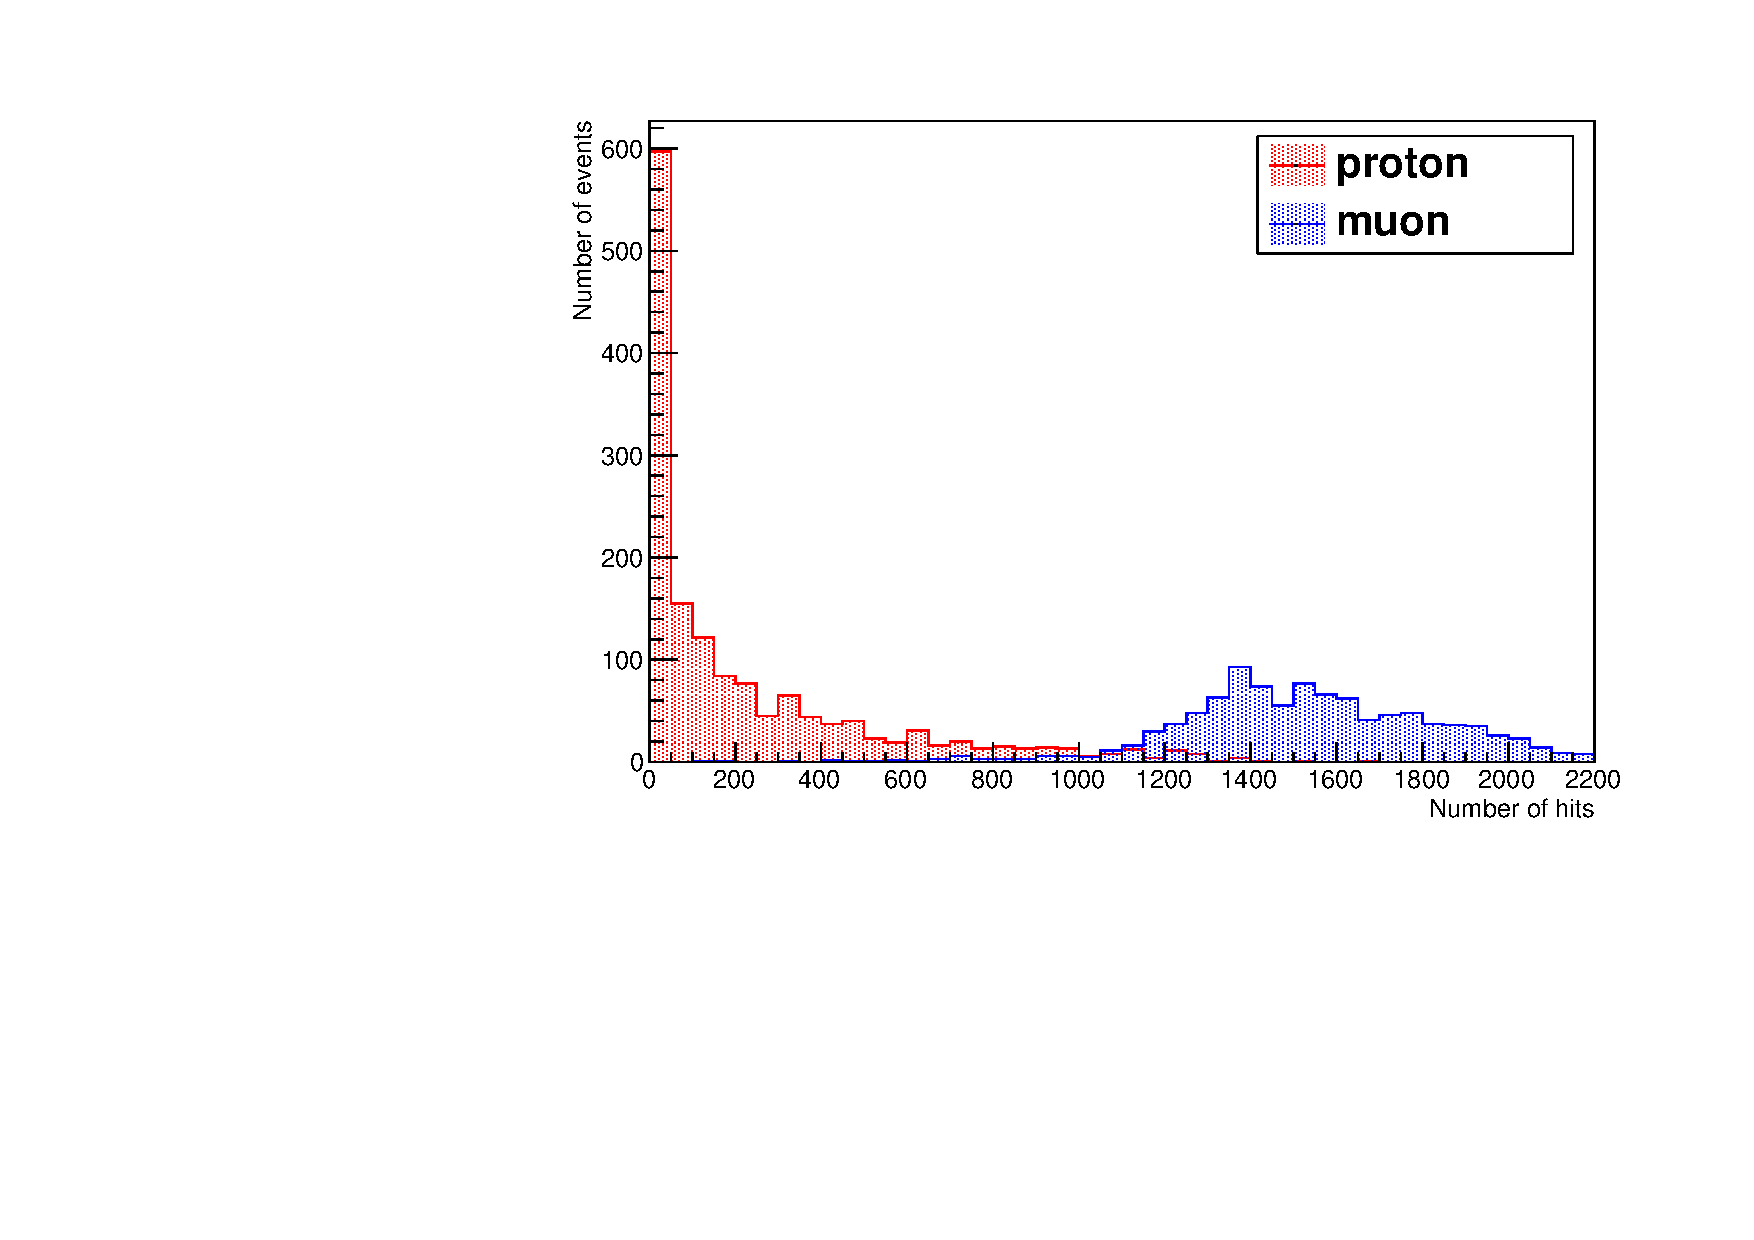
\includegraphics[angle=-90,width=0.8\textwidth]{chapters/particleid_images/particle-lengths-ccqe-770}
\caption[Track length distribution for $\mu$ and $p$ from $770\MeV$ neutrinos (CCQE)]{\label{fig:ccqe-track-lengths-770MeV}Distribution of track lengths, represented as number of hits contained in a track, for muon (blue) and proton (red) tracks produced in charged current interactions of $\nu_\mu$ at $770\MeV$. The distributions are naturally separated at around $1000$ hits.}
\end{figure}

\begin{figure}
\centering
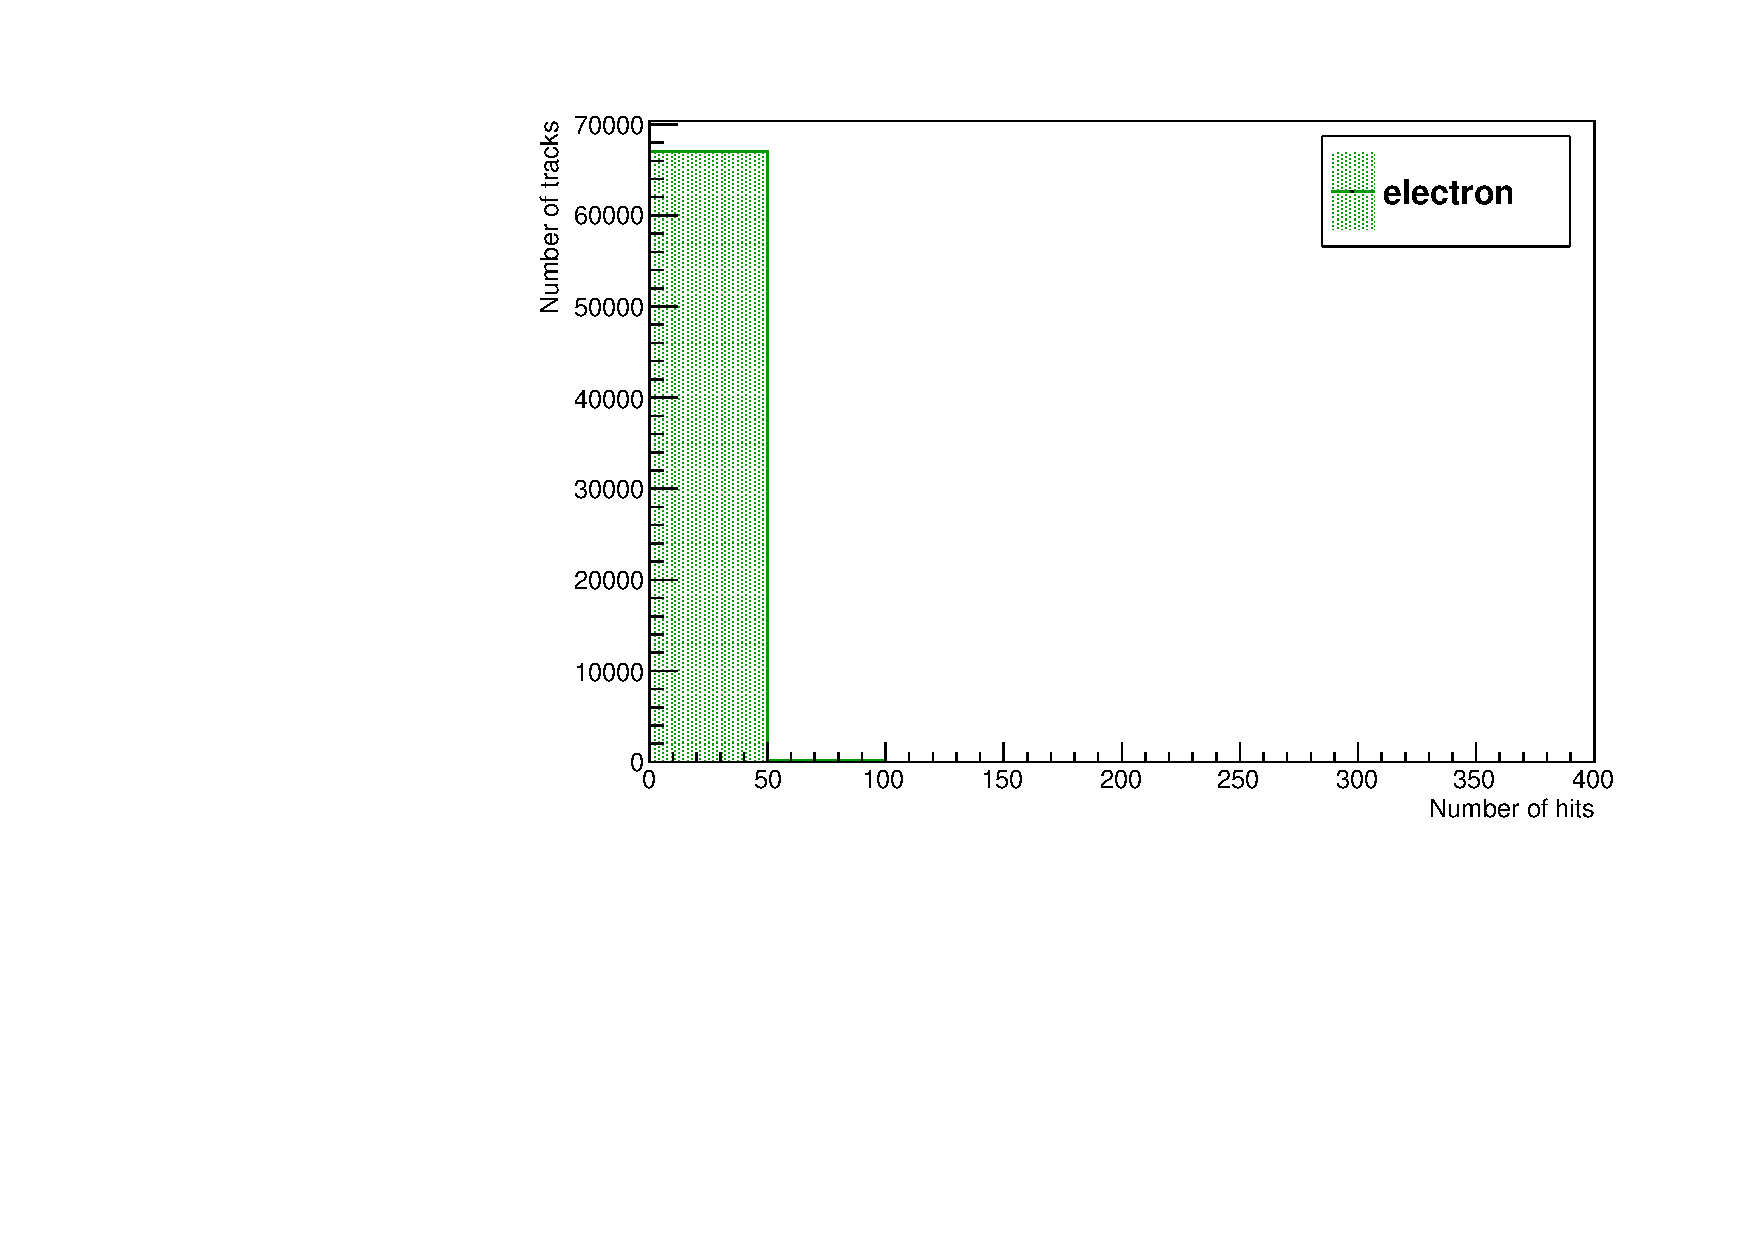
\includegraphics[angle=-90,width=0.8\textwidth]{chapters/particleid_images/electron-lengths-ccqe-770}
\caption[Track length distribution for $e^{-}$ from $770\MeV$ neutrinos (CCQE)]{\label{fig:ccqe-electron-lengths-770MeV}Distribution of track lengths, represented as number of hits contained in a track, for electron tracks produced as secondary particles following charged current interactions of $\nu_\mu$ at $770\MeV$. An extremely large number of very short electron tracks can be seen, corresponding to the production of delta electrons along the length of the trajectories of the primary muon and proton. Most electron tracks have fewer than 50 hits.}
\end{figure}


\clearpage
% ************ 0.77 GeV CCPi ************
\subsection{$770\MeV$ $\nu_\mu \rightarrow \ccpi$ (\acs{CCPi}) Interactions}
This data set contains 1000 events where a $770\MeV$ $\nu_\mu$ underwent a charged current interaction with an Argon nucleus, producing a $\ccpi$ final state. The distribution of track lengths (represented in terms of the number of hits) for muons, protons and charged pions is shown in figure \ref{fig:ccpi-track-lengths-770MeV}. Here, the separation of muons from other particles by track length alone is not a realistic proposal; although the muons dominate the longer tracks, a number of pion tracks are also long enough to provide significant pollution of the muon selection if track length alone is used to discriminate particle type.

\begin{figure}
\centering
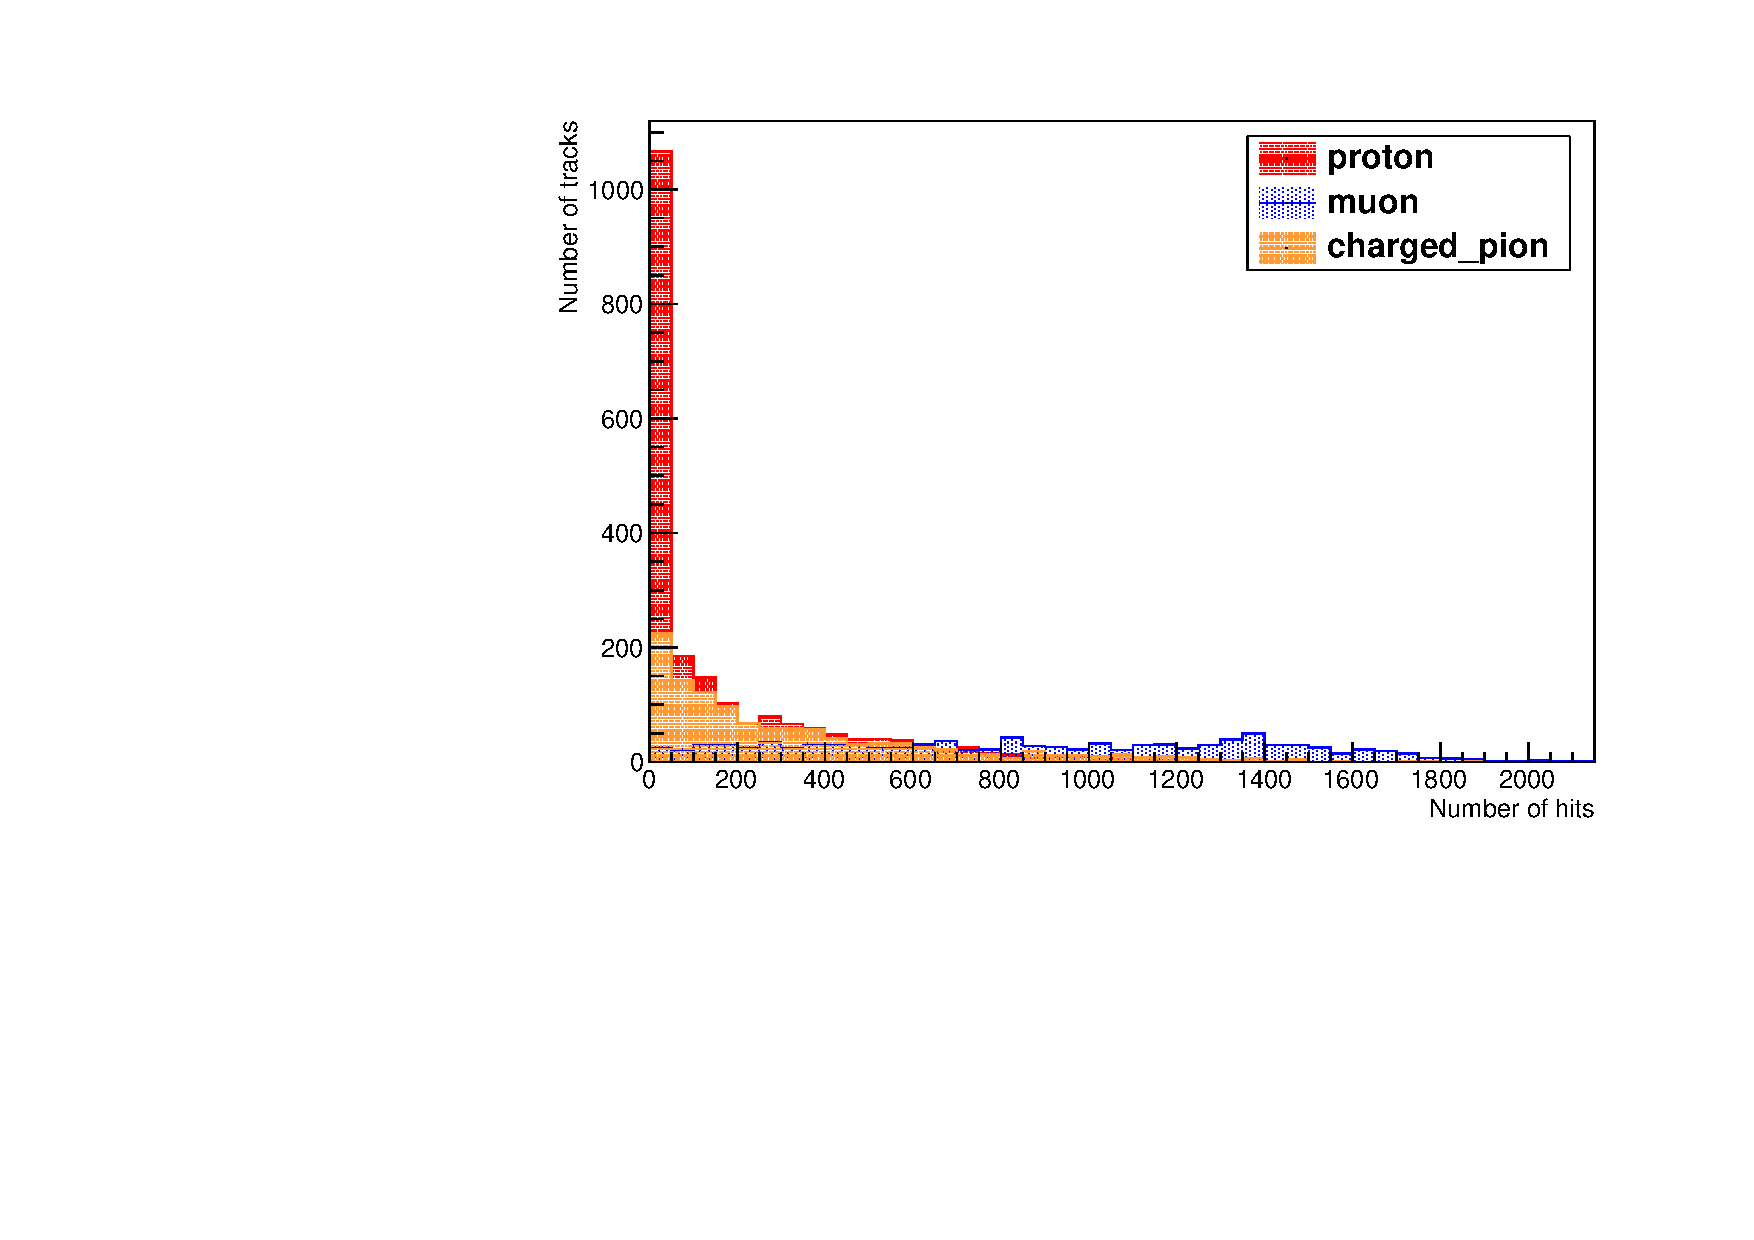
\includegraphics[angle=-90,width=0.8\textwidth]{chapters/particleid_images/ccpi-770-track-lengths}
\caption[Track length distribution for $\mu$, $p$ and $\pi^+$ from $770\MeV$ neutrinos (\acs{CCPi})]{\label{fig:ccpi-track-lengths-770MeV}Distribution of track lengths, represented as number of hits contained in a track, for muon (blue) and proton (red) tracks produced in charged current interactions of $\nu_\mu$ at $770\MeV$ resulting in $\ccpi$ final states. More than $1000$ proton tracks are present, indicating that the $\pi^+$ sometimes produces one or more protons. The distributions are not clearly separated, and while muon tracks are still typically long, there is much more contamination from the other particle species.}
\end{figure}

\clearpage
% ************ 4.5 GeV CCQE ************
\subsection{$4.5\GeV$ $\nu_\mu \rightarrow \ccqe$ (CCQE) Interactions}
This data set contains $10^4$ events in which a $4.5\GeV$ $\nu_\mu$ underwent a charged current interaction with an Argon nucleus, producing a $\ccqe$ final state. The distribution of track lengths (represented in terms of the number of hits) for muons, protons and charged pions (which are produced as secondary particles, in these events) is shown in figure \ref{fig:ccqe-track-lengths-4500MeV}. In addition, a large number of short electron tracks are present, the longest containing only $1238$ hits (in contrast, the muon peak is at 22000 hits).

For these high energy events, it is clear that any track with more than around 5000 hits must correspond to a muon, and the vast majority of muon tracks have between 14000 and 24000 hits. Using the track length to separate muons from other particles should provide an extremely pure selection of muons, in this case. Table \ref{table:cut-results-ccqe-4.5} shows the number of tracks included and excluded by a 5000 hit cut, where the track type is determined from truth information.

\begin{figure}
\centering
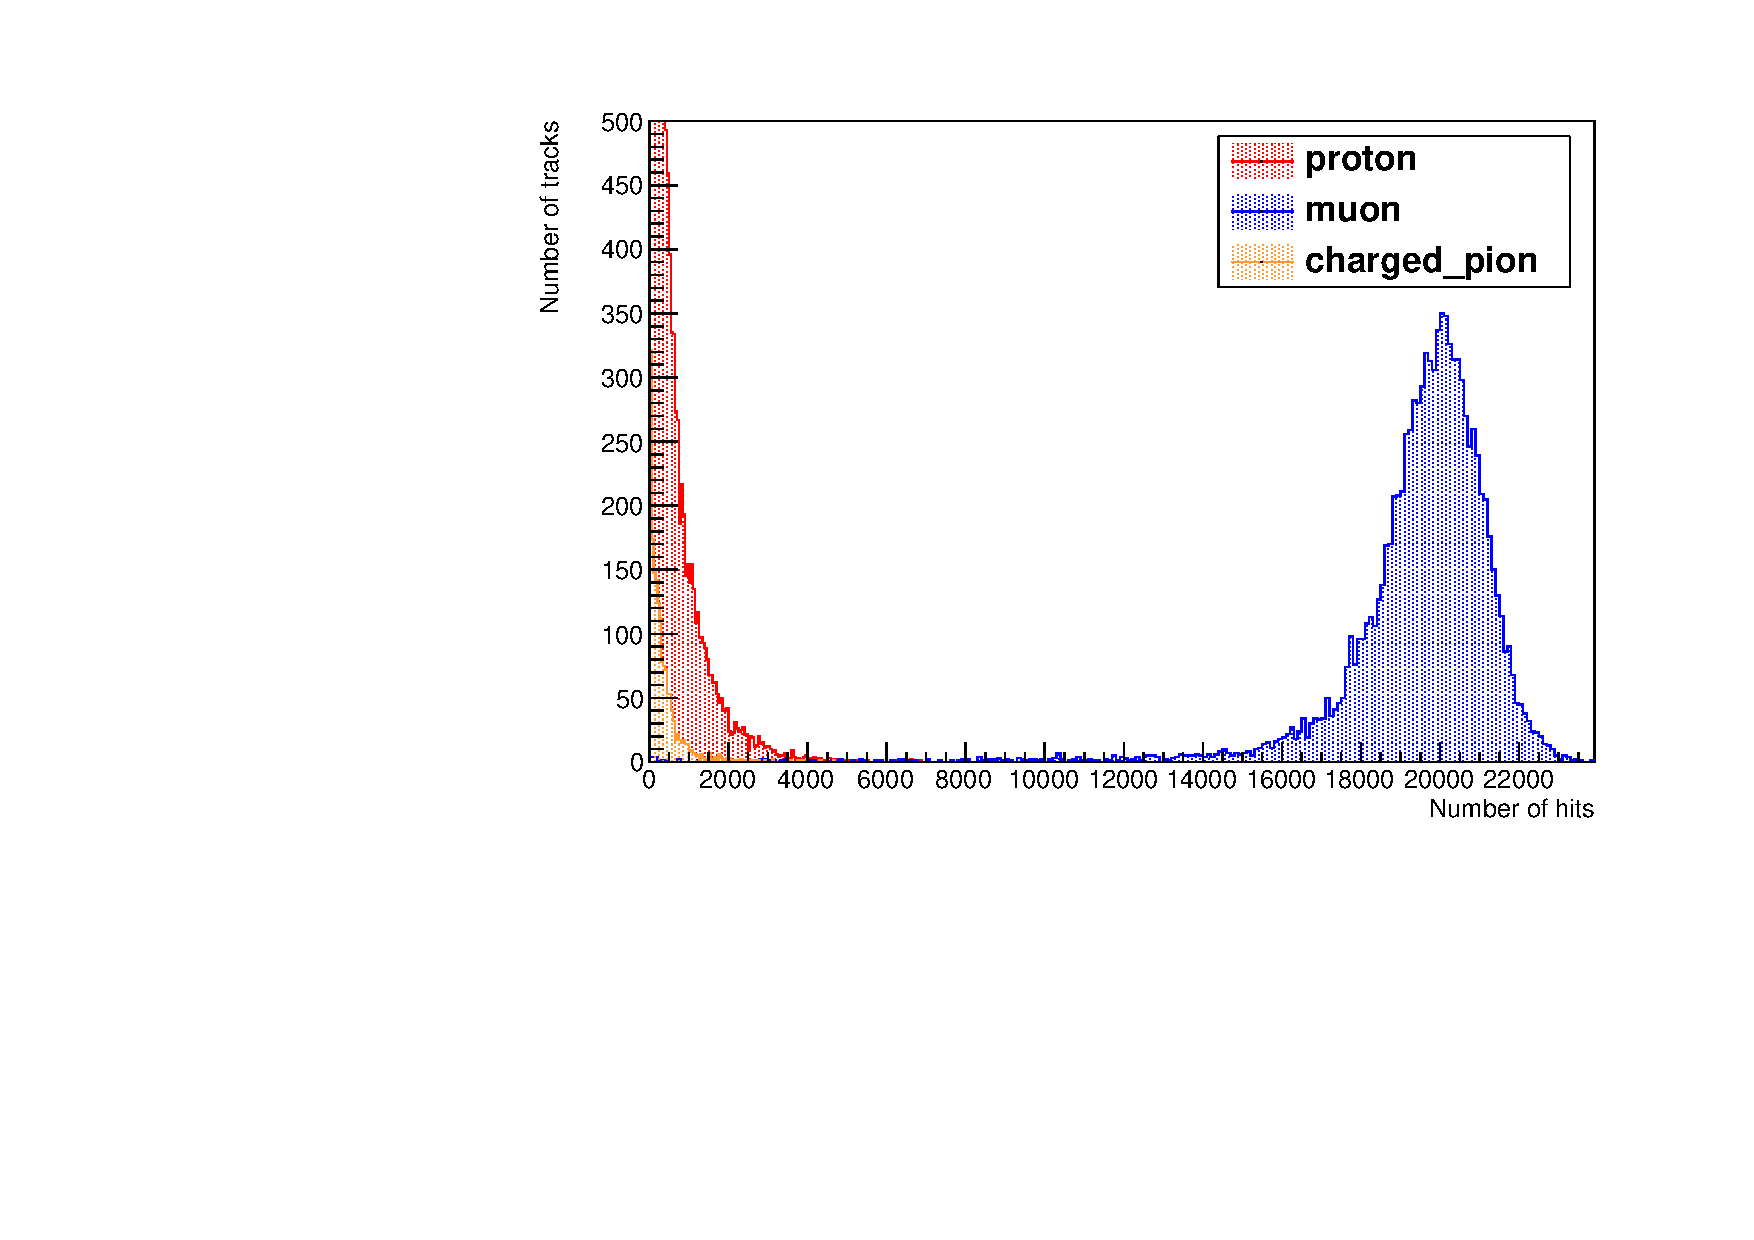
\includegraphics[angle=-90,width=0.8\textwidth]{chapters/particleid_images/ccqe-4500-track-lengths}
\caption[Track length distributions for $\mu$, $p$ and $\pi^+$ from $4.5\GeV$ neutrinos (CCQE)]{\label{fig:ccqe-track-lengths-4500MeV}Distribution of track lengths, represented as number of hits contained in a track, for muon (blue), proton (red) and charged pion (orange) tracks produced in charged current interactions of $\nu_\mu$ at $4.5\GeV$ resulting in $\ccqe$ final states. The proton distribution peaks at over $1.55\times10^4$ tracks on the left.}
\end{figure}

\begin{table}
\centering
\begin{tabular}{*{5}{r}}
 & $\mu$ & $p$ & $e^-$ & $\pi^\pm$ \\
\hline
\hline
Included & 9982 & 14 & 0 & 0 \\
Excluded & 32 & 29640 & 11961433 & 1646 \\
\hline
\end{tabular}
\caption[Composition of tracks after $5000$ hit cut on $4.5\GeV$ CCQE events]{\label{table:cut-results-ccqe-4.5}Composition of tracks after applying a $5000$ hit cut on the truth tracks from simulation of $4.5\GeV$ $\nu_\mu$ interactions producing $\ccqe$ final states. The cut selects muon tracks with $99.7\pm0.1\%$ efficiency and $99.9\pm0.1\%$ purity.}
\end{table}

% ************ 4.5 GeV CCPi ************
\subsection{$4.5\GeV$ $\nu_\mu \rightarrow \ccpi$ (\acs{CCPi}) Interactions}
This data set contains $10^4$ events in which a $4.5\GeV$ $\nu_\mu$ underwent a charged current interaction with an Argon nucleus, producing a $\ccpi$ final state. The distribution of track lengths (represented in terms of the number of hits) for muons, protons and charged pions is shown in figure \ref{fig:ccpi-track-lengths-4500MeV}. The $\pi^+$ and $p$ peaks on the left extend up to $4.3\times10^4$ tracks. In this case, the muons are once again clearly separated, as for the CCQE events at $4.5\GeV$, and a cut at 5000 hits would select almost entirely muon tracks, rejecting those from protons and pions. Table \ref{table:cut-results-ccpi-4.5} shows the number of included and excluded tracks following a 5000 hit cut.

\begin{figure}
\centering
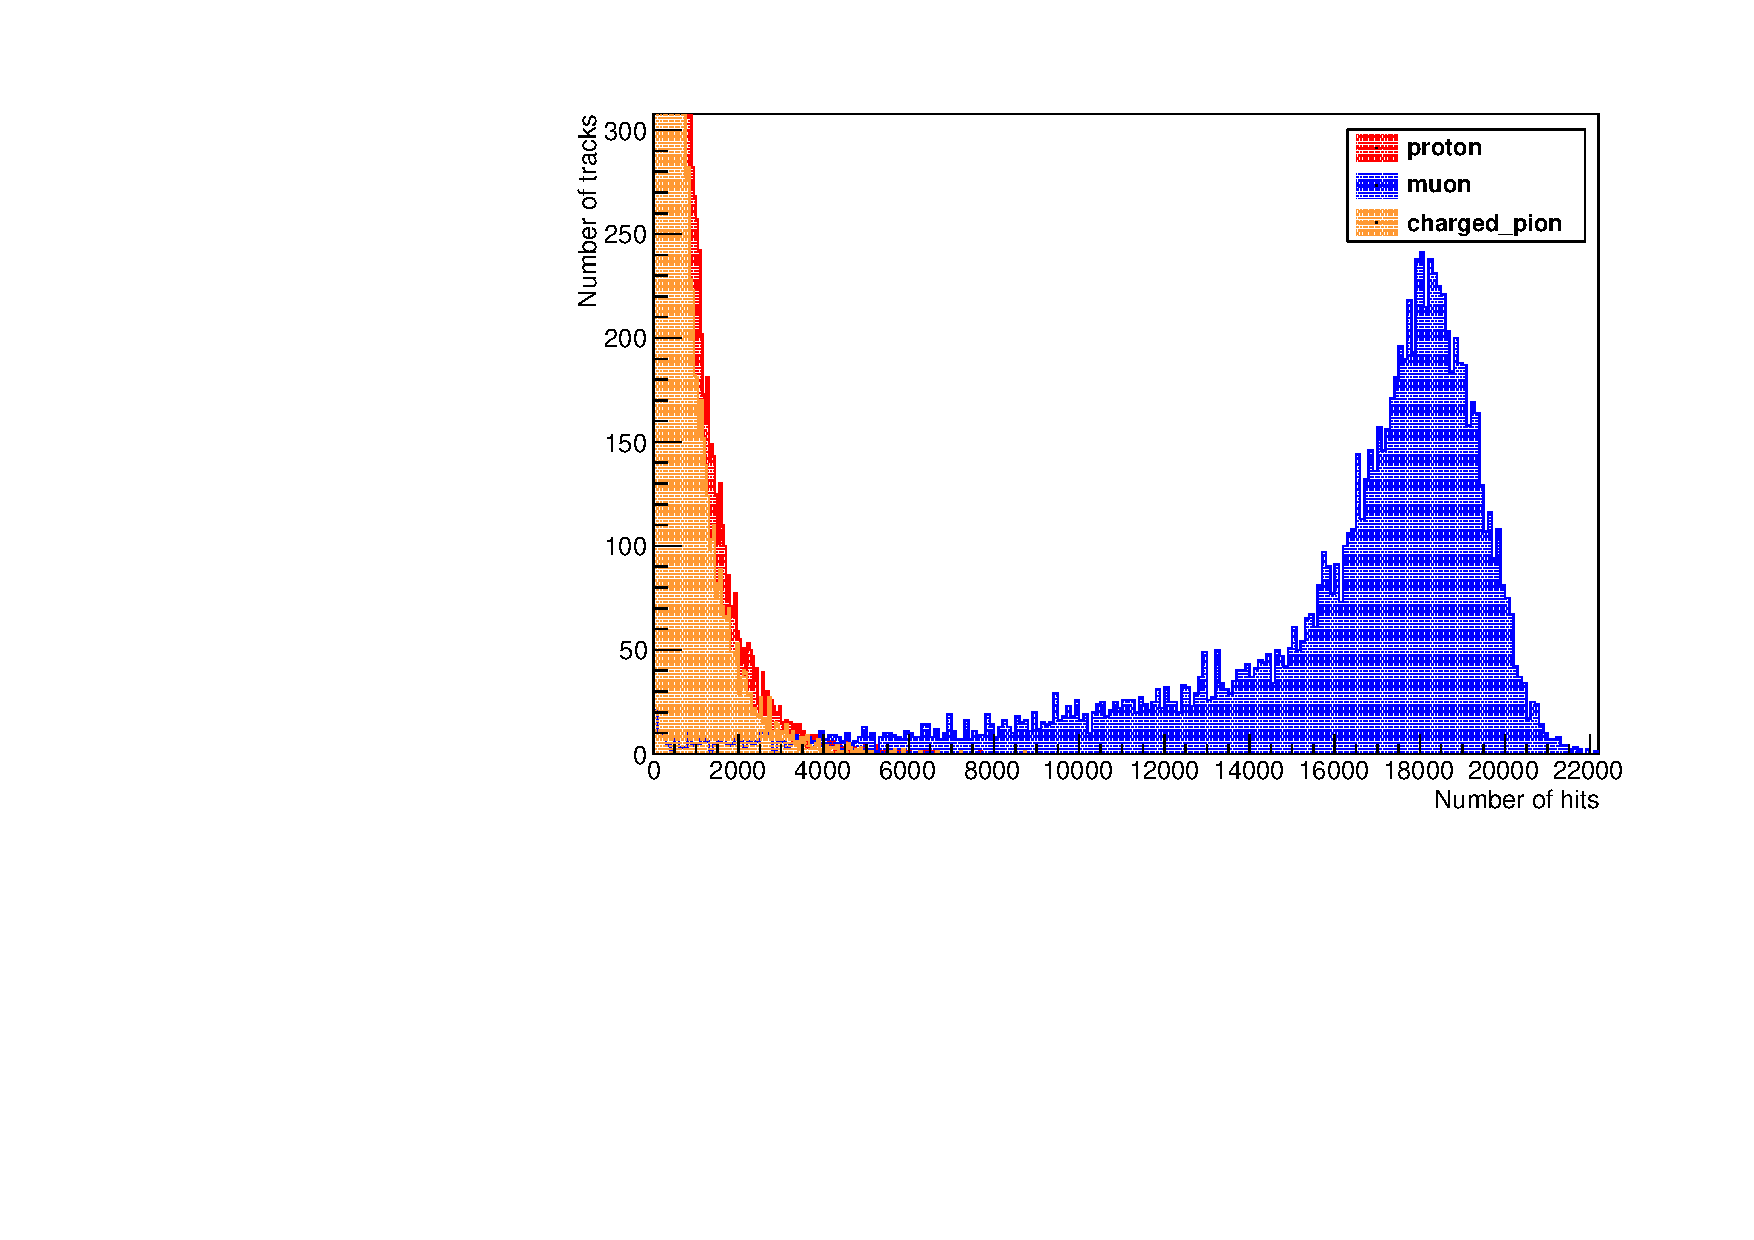
\includegraphics[angle=-90,width=0.8\textwidth]{chapters/particleid_images/tracks-ccpi-4500MeV}
\caption[Track length distribution for $\mu$, $p$ and $\pi^+$ from $4.5\GeV$ neutrinos (\acs{CCPi})]{\label{fig:ccpi-track-lengths-4500MeV}Distribution of track lengths, represented as number of hits contained in a track, for muon (blue), proton (red) and charged pion (orange) tracks produced in charged current interactions of $\nu_\mu$ at $4.5\GeV$, resulting in $\ccpi$ final states. The proton and pion peaks on the left extend up to $4.3\times10^4$, and the plot range has been reduced to better display the separation between hadron ($p$ and $\pi$) and lepton ($\mu$) tracks. A cut at 5000 hits would cleanly select muons with low contamination from other tracks.}
\end{figure}

\begin{table}
\centering
\begin{tabular}{*{6}{r}}
 & $\mu$ & $p$ & $e^-$ & $\pi^\pm$ & Other \\
\hline
\hline
Included & 9717 & 24 & 0 & 12 & 12 \\
Excluded & 337 & 67286 & 12854577 & 18691 & 188995 \\
\hline
\end{tabular}
\caption[Composition of tracks after $5000$ hit cut on $4.5\GeV$ \acs{CCPi} events]{\label{table:cut-results-ccpi-4.5}Composition of tracks after applying a $5000$ hit cut on the truth tracks from simulation of $4.5\GeV$ $\nu_\mu$ interactions producing $\ccpi$ final states. The cut selects muon tracks with $96.6\pm0.2\%$ efficiency and $99.5\pm0.1\%$ purity.}
\end{table}

\clearpage
\subsection{Conclusions}
It is clear from the track distributions presented above that for the low energy $\mu + p$ events, and for the high energy $\ccqe$ and $\ccpi$ events, a simple cut on the minimum track length is sufficient to select muon tracks from an event. The low energy $\ccpi$ events are an exception to this, and present a more complicated case for analysis, which may require further variables to be considered in order to extract muons with high purity. More traditional particle identification mechanisms, which make use of many variables and attempt to categorise events based on likelihood fits or the results of a neural network are not considered here, but may prove useful in cases such as the low energy $\ccpi$, where the interactions of the particles differ considerably, but are not well represented in the track length alone.

For the remaining three event classes (high and low energy CCQE, high energy \acs{CCPi}) this range cut should retain high efficiency, though it is worth noting that the studies in this chapter consider truth information, and that the effects of a reconstruction algorithm such as the cellular automaton of chapter \ref{chapter:CellularAutomaton} will necessarily reduce the efficiency of such a technique. The cut values are summarised in table \ref{table:summary_cuts}.

\begin{table}
\centering
\begin{tabular}{cccc}
Class & Cut Value (Hits) & Efficiency & Purity \\
\hline
\hline
CCQE $770\MeV$ & 1000 & $96.0\pm0.6$ & $94.4\pm0.8$ \\
CCQE $4.5\GeV$ & 5000 & $99.7\pm0.1$ & $99.9\pm0.1$ \\
\acs{CCPi} $4.5\GeV$ & 5000 & $96.6\pm0.2$ & $99.5\pm0.1$ \\
\hline
\end{tabular}
\caption[Summary of cuts with efficiencies and purities]{\label{table:summary_cuts}Summary of the cuts for muon selection in different event classes, including the efficiency for selecting muons, and the resulting purity.}
\end{table}

\section{Angular Distributions}
Relativistic kinematics dictates that the angular distribution of final state particles will depend on their mass~\citep{PDG2012}. Differences in the angular distribution of muons, protons and charged pions could allow for the construction of PID variables to aid the discrimination between those particle species. In this section, a comparison is made between the angular distributions of protons and muons in \acs{CCQE} interactions at $0.77\GeV$ and $4.5\GeV$ energies, and for \acs{CCPi} interactions at the same energies, including the distribution of charged pions.

In each case, the data is taken from the output of a set of Genie interactions, using the following quantities based on the final state particle momentum. Note that these correspond to components of a unit vector along the momentum vector, or, equivalently, normalised direction vectors, i.e. direction cosines $\cos\alpha_{x,y,z}$, with a range between $-1$ and $1$.

\begin{equation}\label{eqn:angular_variables}
    \hat{p}_{x,y,z} = \frac{p_{x,y,z}}{p_x^2 + p_y^2 + p_z^2}
\end{equation}

These interactions were generated with a muon neutrino beam in the $+x$ direction, so the distributions should be peaked in the forward $x$ direction, and symmetric in $y$ and $z$.

\subsection{$770\MeV$ $\nu_\mu \rightarrow \ccqe$ (CCQE) Interactions}
Figure \ref{fig:ccqe-770-angle} shows the angular distribution of muons and protons in \acs{CCQE} $\nu_\mu$ interactions at $770\MeV$, producing a $\ccqe$ final state. The distributions are almost identical, which does not permit a simple cut value to be selected for PID discrimination and would likely be problematic for a multivariate analysis using e.g. TMVA~\citep{TMVA} to combine several discriminators. Separation of muons and protons from \acs{CCQE} interactions at low energy ($770\MeV$) using angular information alone is, therefore, not practical.

\begin{figure}
    \centering
    \subfigure[$\hat{p}_x$]{
        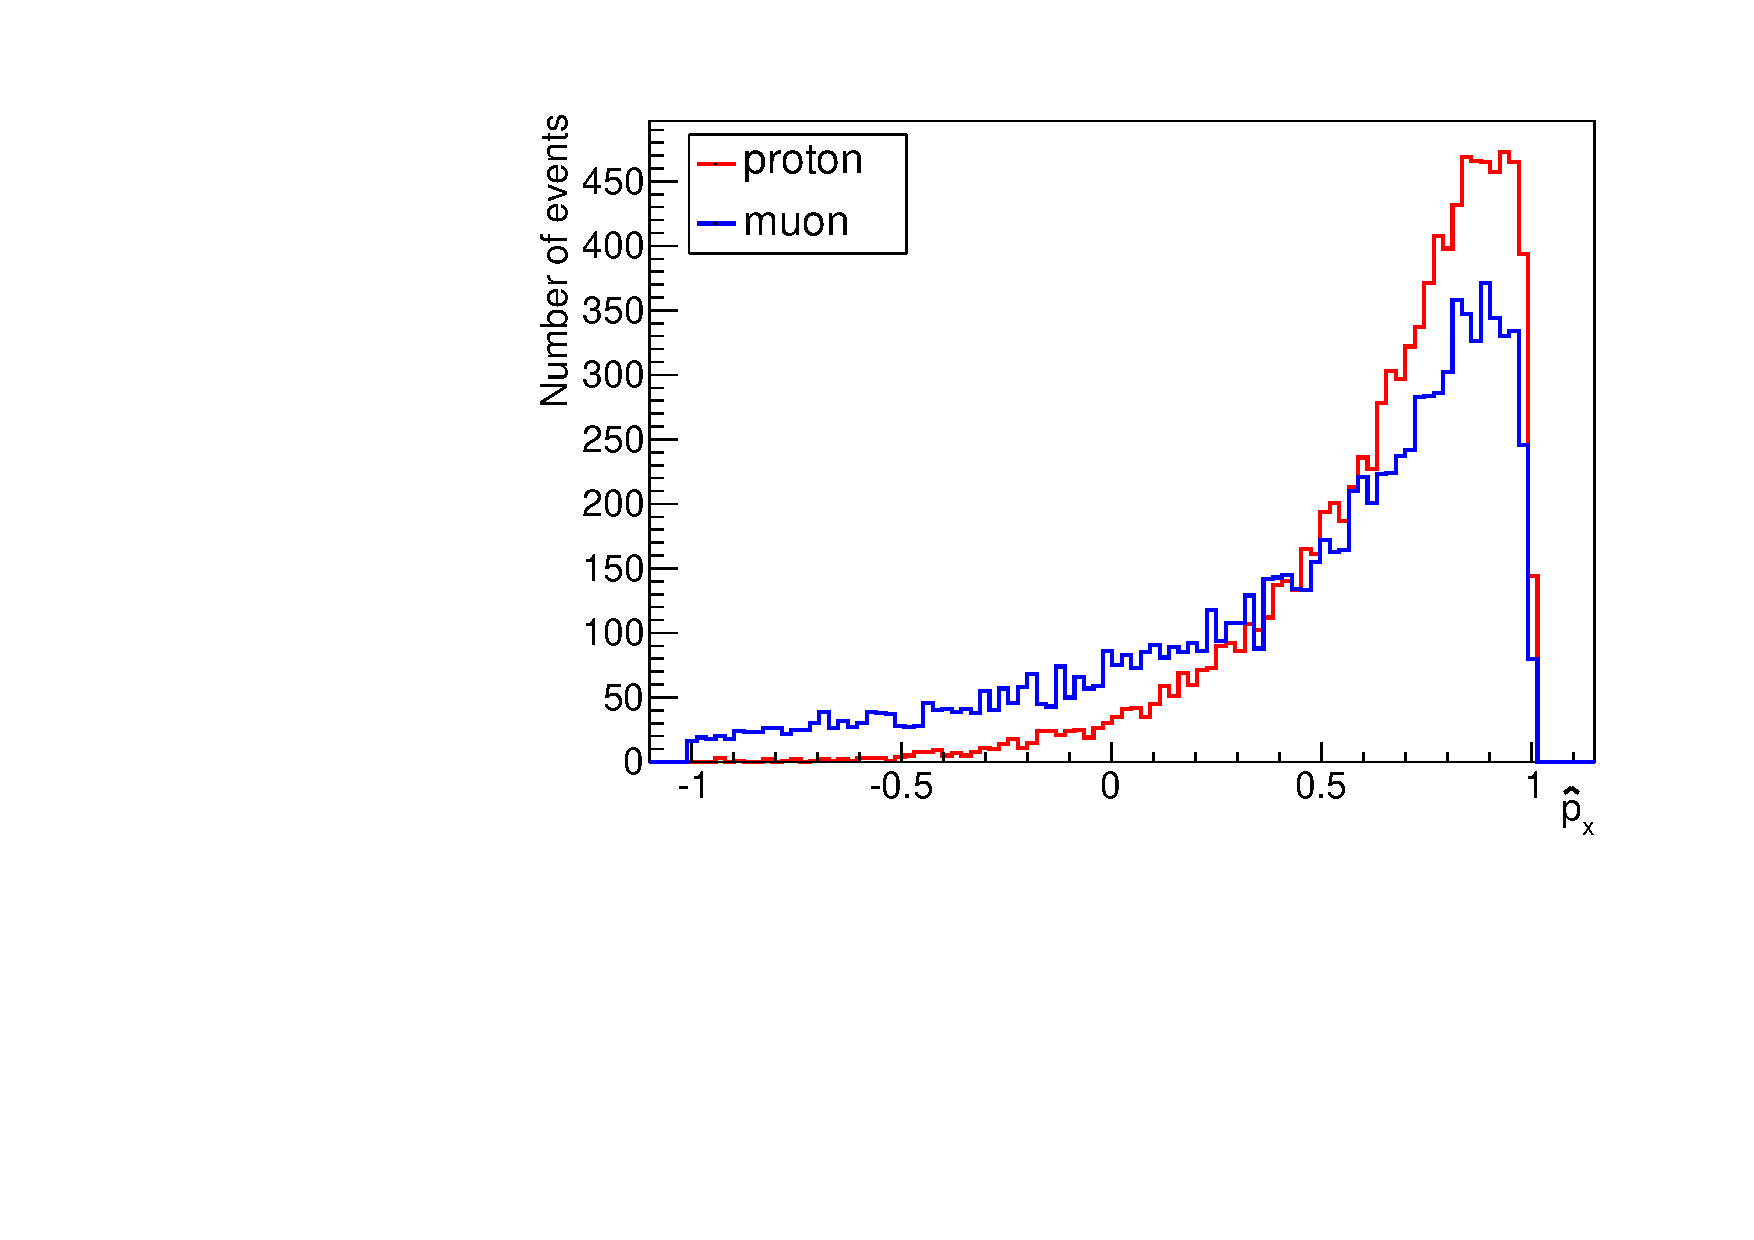
\includegraphics[angle=-90,width=0.65\textwidth]{chapters/particleid_images/ccqe-px-770}
        \label{fig:ccqe-px-770}
    }
    \subfigure[$\hat{p}_y$]{
        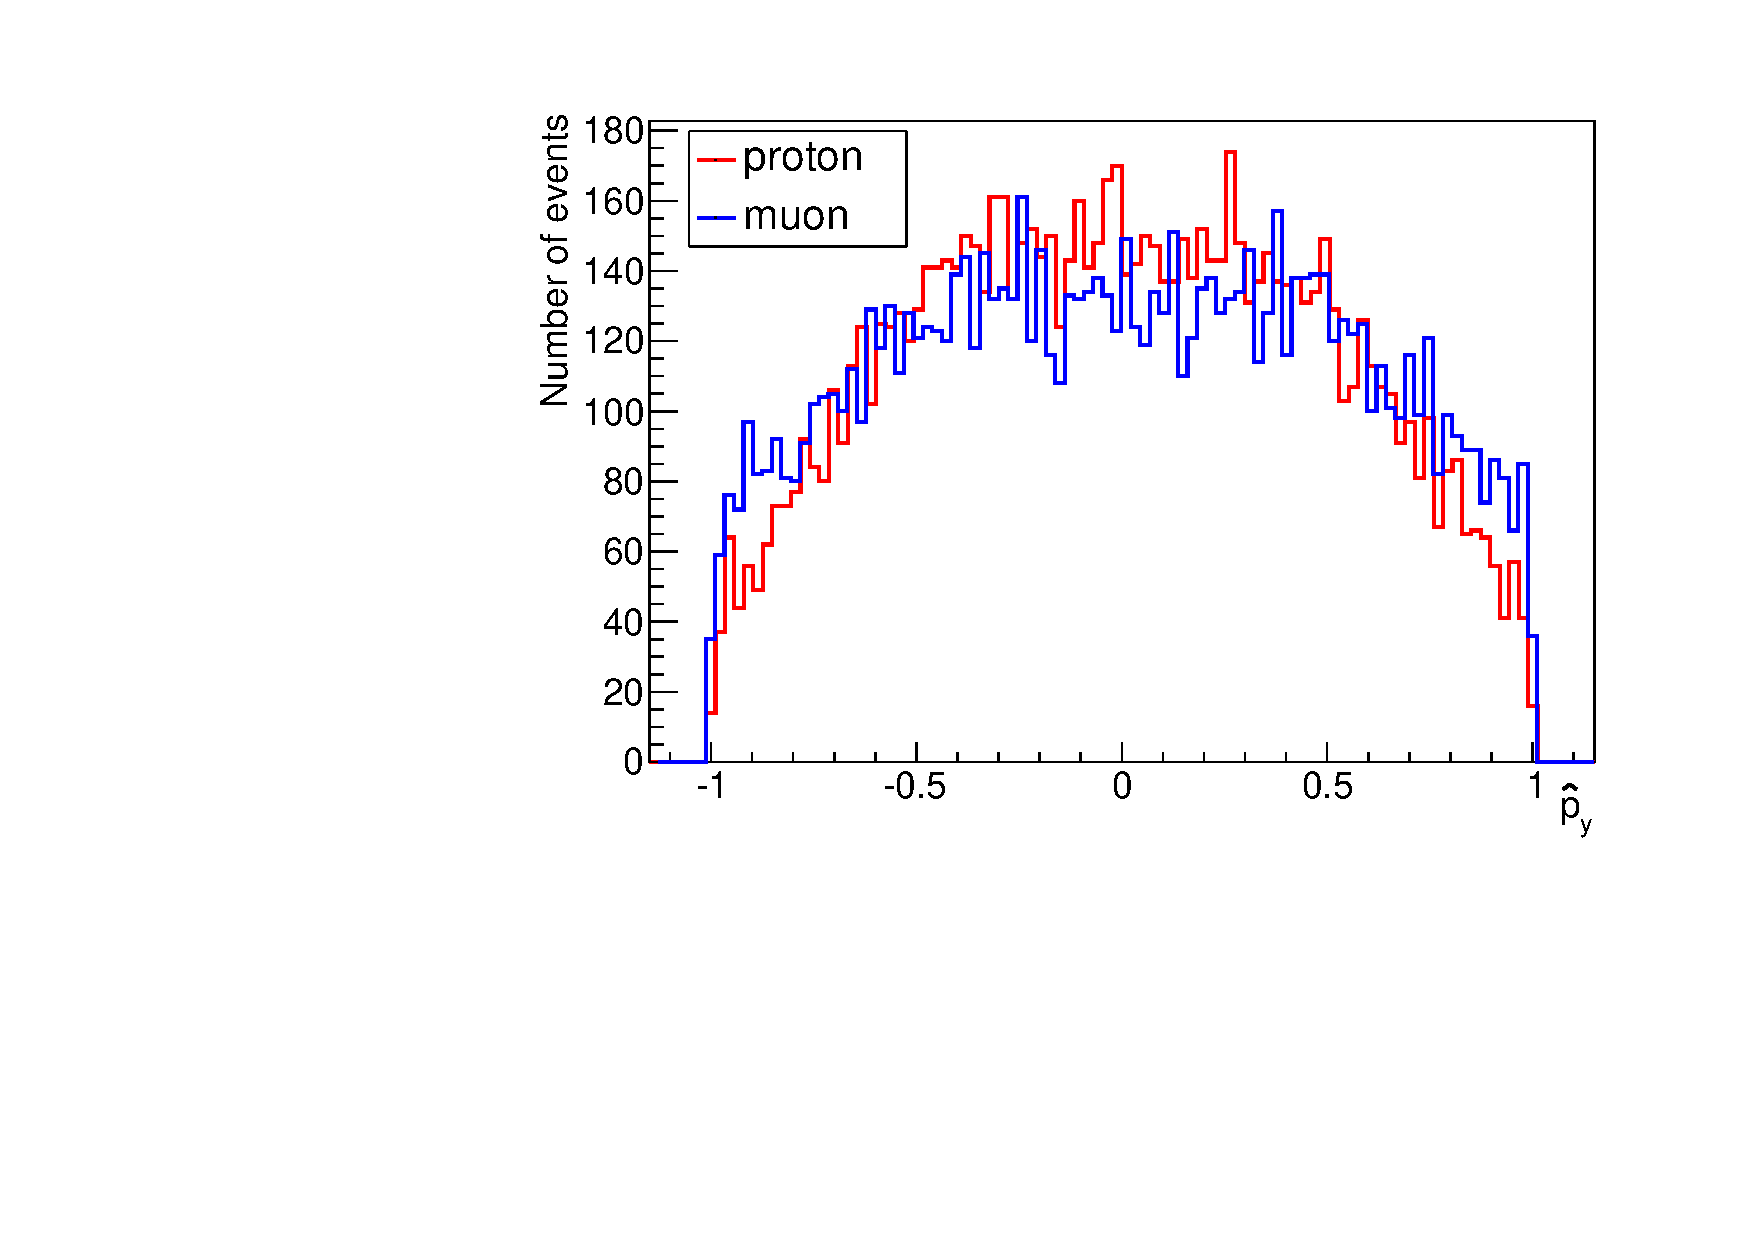
\includegraphics[angle=-90,width=0.65\textwidth]{chapters/particleid_images/ccqe-py-770}
        \label{fig:ccqe-py-770}
    }
    \subfigure[$\hat{p}_z$]{
        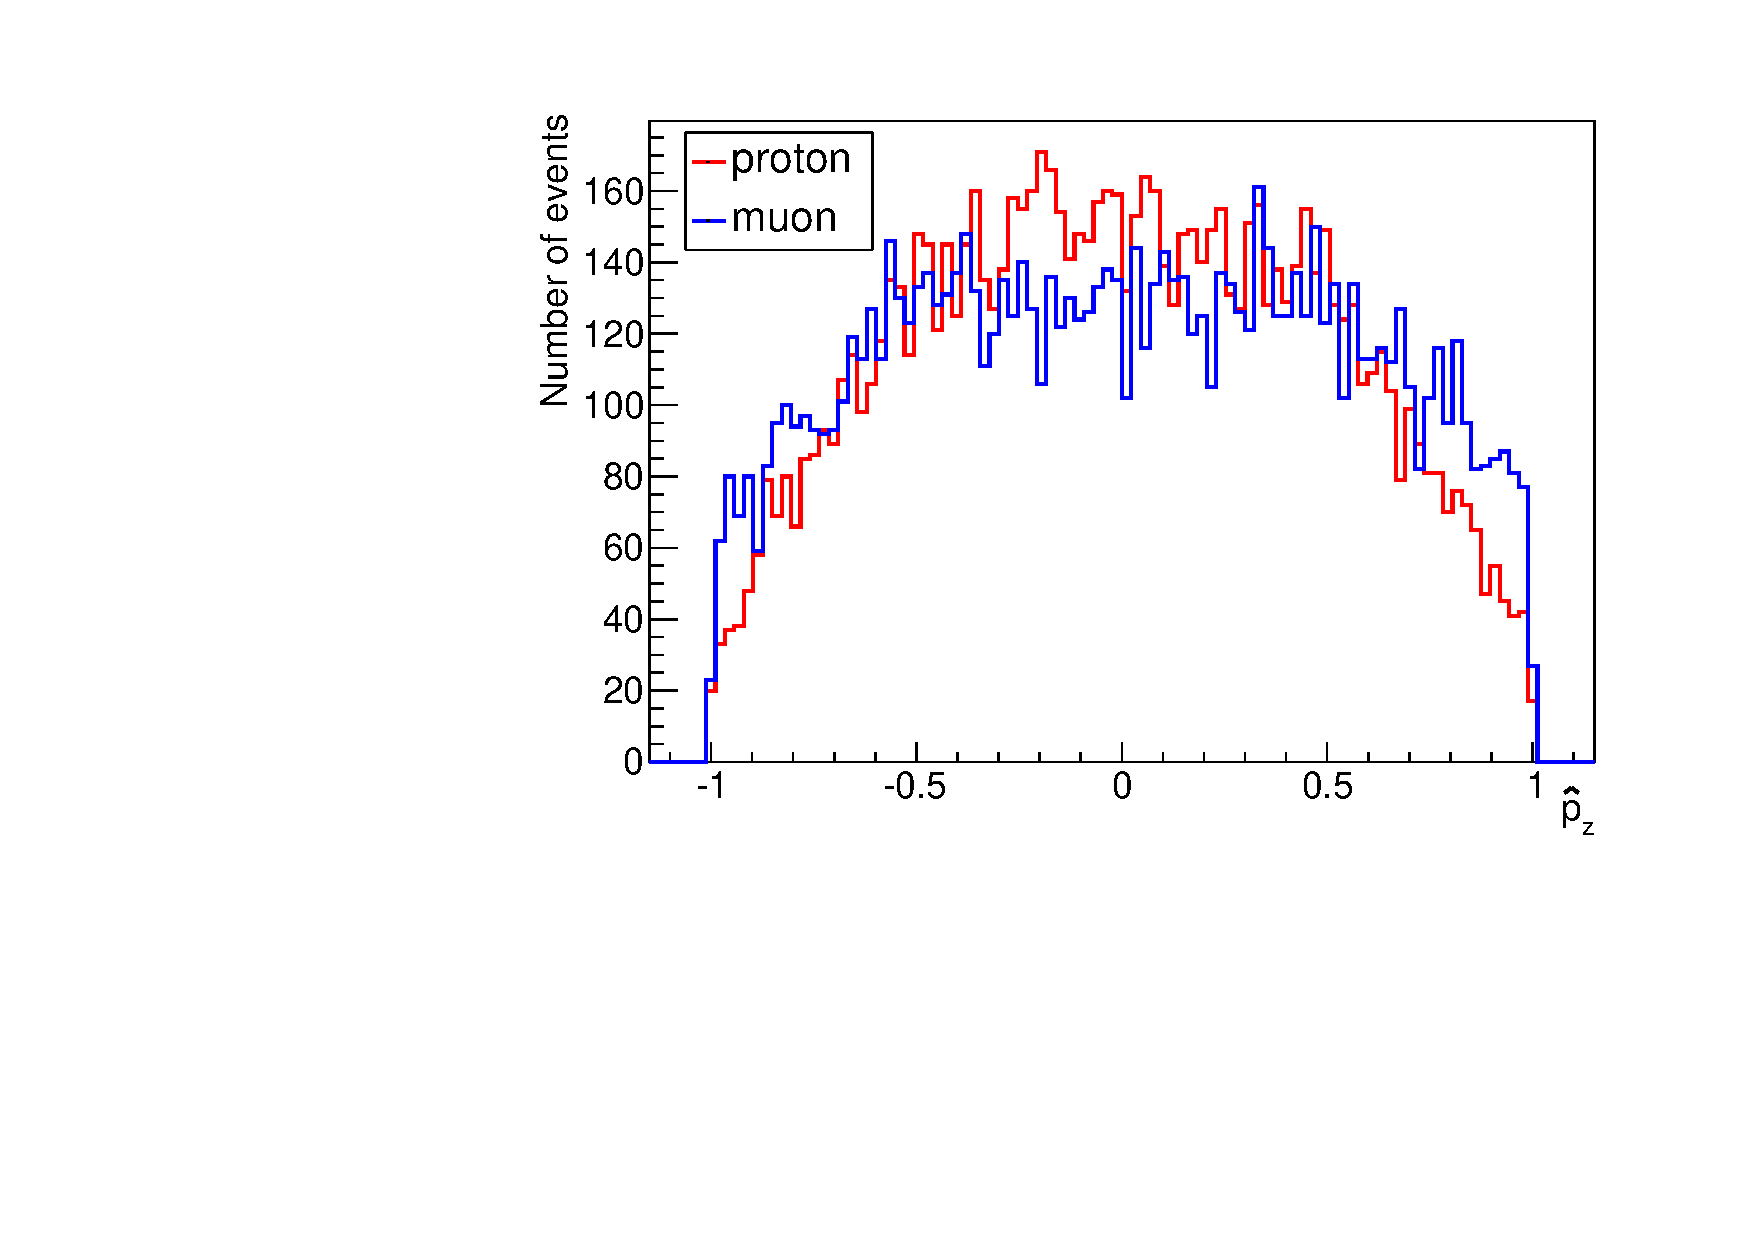
\includegraphics[angle=-90,width=0.65\textwidth]{chapters/particleid_images/ccqe-pz-770}
        \label{fig:ccqe-pz-770}
    }
    \caption[Angular distribution of $\mu$, $p$ at $770\MeV$]{\label{fig:ccqe-770-angle}Angular distribution of muons and protons in \acs{CCQE} interactions at $770\MeV$. See text for discussion.}
\end{figure}

\subsection{$770\MeV$ $\nu_\mu \rightarrow \ccpi$ (\acs{CCPi}) Interactions}

\subsection{$4.5\GeV$ $\nu_\mu \rightarrow \ccqe$ (CCQE) Interactions}

\subsection{$4.5\GeV$ $\nu_\mu \rightarrow \ccpi$ (\acs{CCPi}) Interactions}
